% Options for packages loaded elsewhere
% Options for packages loaded elsewhere
\PassOptionsToPackage{unicode,bookmarks=true,bookmarksopen=true,bookmarksnumbered=true,pdfpagemode=UseOutlines,pdftoolbar=true,pdfmenubar=true,pdffitwindow=false,pdfstartview=FitH,colorlinks=true,linktocpage=false}{hyperref}
\PassOptionsToPackage{hyphens}{url}
\PassOptionsToPackage{dvipsnames,svgnames,x11names}{xcolor}
%
\documentclass[
  onepage,
  openany]{scrbook}
\usepackage{xcolor}
\usepackage[top=25mm,bottom=35mm,left=25mm,right=25mm,heightrounded]{geometry}
\usepackage{amsmath,amssymb}
\setcounter{secnumdepth}{3}
\usepackage{iftex}
\ifPDFTeX
  \usepackage[T1]{fontenc}
  \usepackage[utf8]{inputenc}
  \usepackage{textcomp} % provide euro and other symbols
\else % if luatex or xetex
  \usepackage{unicode-math} % this also loads fontspec
  \defaultfontfeatures{Scale=MatchLowercase}
  \defaultfontfeatures[\rmfamily]{Ligatures=TeX,Scale=1}
\fi
\usepackage{lmodern}
\ifPDFTeX\else
  % xetex/luatex font selection
\fi
% Use upquote if available, for straight quotes in verbatim environments
\IfFileExists{upquote.sty}{\usepackage{upquote}}{}
\IfFileExists{microtype.sty}{% use microtype if available
  \usepackage[]{microtype}
  \UseMicrotypeSet[protrusion]{basicmath} % disable protrusion for tt fonts
}{}
\makeatletter
\@ifundefined{KOMAClassName}{% if non-KOMA class
  \IfFileExists{parskip.sty}{%
    \usepackage{parskip}
  }{% else
    \setlength{\parindent}{0pt}
    \setlength{\parskip}{6pt plus 2pt minus 1pt}}
}{% if KOMA class
  \KOMAoptions{parskip=half}}
\makeatother
% Make \paragraph and \subparagraph free-standing
\makeatletter
\ifx\paragraph\undefined\else
  \let\oldparagraph\paragraph
  \renewcommand{\paragraph}{
    \@ifstar
      \xxxParagraphStar
      \xxxParagraphNoStar
  }
  \newcommand{\xxxParagraphStar}[1]{\oldparagraph*{#1}\mbox{}}
  \newcommand{\xxxParagraphNoStar}[1]{\oldparagraph{#1}\mbox{}}
\fi
\ifx\subparagraph\undefined\else
  \let\oldsubparagraph\subparagraph
  \renewcommand{\subparagraph}{
    \@ifstar
      \xxxSubParagraphStar
      \xxxSubParagraphNoStar
  }
  \newcommand{\xxxSubParagraphStar}[1]{\oldsubparagraph*{#1}\mbox{}}
  \newcommand{\xxxSubParagraphNoStar}[1]{\oldsubparagraph{#1}\mbox{}}
\fi
\makeatother


\usepackage{longtable,booktabs,array}
\usepackage{calc} % for calculating minipage widths
% Correct order of tables after \paragraph or \subparagraph
\usepackage{etoolbox}
\makeatletter
\patchcmd\longtable{\par}{\if@noskipsec\mbox{}\fi\par}{}{}
\makeatother
% Allow footnotes in longtable head/foot
\IfFileExists{footnotehyper.sty}{\usepackage{footnotehyper}}{\usepackage{footnote}}
\makesavenoteenv{longtable}
\usepackage{graphicx}
\makeatletter
\newsavebox\pandoc@box
\newcommand*\pandocbounded[1]{% scales image to fit in text height/width
  \sbox\pandoc@box{#1}%
  \Gscale@div\@tempa{\textheight}{\dimexpr\ht\pandoc@box+\dp\pandoc@box\relax}%
  \Gscale@div\@tempb{\linewidth}{\wd\pandoc@box}%
  \ifdim\@tempb\p@<\@tempa\p@\let\@tempa\@tempb\fi% select the smaller of both
  \ifdim\@tempa\p@<\p@\scalebox{\@tempa}{\usebox\pandoc@box}%
  \else\usebox{\pandoc@box}%
  \fi%
}
% Set default figure placement to htbp
\def\fps@figure{htbp}
\makeatother





\setlength{\emergencystretch}{3em} % prevent overfull lines

\providecommand{\tightlist}{%
  \setlength{\itemsep}{0pt}\setlength{\parskip}{0pt}}



 


% This is an UHH LaTeX template for a Quarto PDF document.

% -----------------------------------------------------
% --- FORMAT STYLE FOR KOMA DOCUMENT CLASS SCRBOOK ---
% -----------------------------------------------------


% %----------------------------------------------- General format

\usepackage[T1]{fontenc}
\usepackage[utf8]{inputenc}
\usepackage{hyphenat}

% For title page
\usepackage{afterpage}  
\usepackage{tikz}
\usetikzlibrary{fadings}
\usepackage[pagecolor=none]{pagecolor}

% Paragraph settings {{{
\setlength{\parindent}{0em}           %  indentation at the first line of a paragraph (here set to 0)
\setlength{\parskip}{0.5em}             % paragraph spacing
\renewcommand{\baselinestretch}{1.0}    % line spacing (here single)
% }}}


% %----------------------------------------------- Fonts

\usepackage{anyfontsize}

% General {{{
\defaultfontfeatures{Mapping = tex-text}
\setmainfont[BoldFont = font_bold.ttf, ItalicFont = font_italic.ttf, BoldItalicFont = font_bolditalic.ttf]{font_regular.ttf}
\newfontfamily\headingfont[ItalicFont = font_bolditalic.ttf]{font_bold.ttf}
% }}}

% Title and header {{{
\setkomafont{title}{\rmfamily\huge\bfseries}
\setkomafont{subtitle}{\rmfamily\Large}
\setkomafont{author}{\rmfamily\large\bfseries}
\setkomafont{date}{\rmfamily\small\bfseries}
\setkomafont{sectioning}{\rmfamily\large\bfseries}
% }}}

% setting caption text
\usepackage[font=small,labelfont=bf]{caption}



% %----------------------------------------------- Colors

\usepackage{xcolor}				% extends LATEX's color facilities
\usepackage{colortbl}			% to add colour to LaTeX tables
\usepackage{hyperref}			% to handle cross-referencing commands in LaTeX
\PassOptionsToPackage{dvipsnames,svgnames*,x11names*}{xcolor} % for colorlinks

% Define colors for headers and links: {{{
\definecolor{bluegray}{HTML}{3B515B} 
\definecolor{blue}{HTML}{0271BB} 
% }}}

% Font colors {{{
\addtokomafont{title}{\color{bluegray}}           % text color for title
\addtokomafont{subtitle}{\color{bluegray}}        % text color for subtitle
\addtokomafont{author}{\color{bluegray}}          % text color for author
\addtokomafont{date}{\color{bluegray}}            % text color for date
\addtokomafont{disposition}{\color{bluegray}}     % text color for toc section header
\addtokomafont{section}{\color{blue}}             % text color for section header
\addtokomafont{subsection}{\color{bluegray}}      % text color for subsection header
\addtokomafont{subsubsection}{\color{bluegray}}   % text color for subsubsection header
% }}}

% Hypersetup for links {{{ --> currently not working!
\hypersetup{
colorlinks=true,
linkcolor=linkcol,
filecolor=linkcol,
urlcolor=linkcol,
citecolor=linkcol,
bookmarks=true,
linktocpage=true,
pdfpagemode=UseOutlines
}
% }}}


% %----------------------------------------------- Header and footer

% Delete default settings and define your own {{{
\usepackage[headsepline, automark]{scrlayer-scrpage}
\clearpairofpagestyles
\ohead[]{\headmark} 
\ofoot[\pagemark]{\pagemark}
% \ifoot[]{
\includegraphics[height=10mm]{uhh_logo.png}}
% }}}



% %----------------------------------------------- Lists

% Itemized lists {{{
\renewcommand{\labelitemi}{\tiny\textcolor{blue}{$\blacksquare$}}
\renewcommand{\labelitemii}{\textcolor{bluegray}{$\bullet$}}
\renewcommand{\labelitemiii}{\textcolor{blue}{$\bullet$}}
\renewcommand{\labelitemiv}{\textcolor{bluegray}{$\bullet$}}
% }}}

% Enumerated lists {{{ --> does not work currently
% \renewcommand{\theenumi}{\color{blue}}
% \renewcommand{\theenumii}{\color{bluegray}}
% \renewcommand{\theenumiii}{\textcolor{blue}}
% \renewcommand{\theenumiv}{\textcolor{bluegray}}
% }}}



% %----------------------------------------------- Graphics

\usepackage{graphicx}
\graphicspath{ {images/} } % images have to be in the /image subfolder
\usepackage{picture}
% Make entire TOC entries clickable, not just page numbers
\hypersetup{
  linktocpage=false,
  linktoc=all
}
% Prevent blank pages before chapters
\KOMAoptions{twoside=false}
\raggedbottom
\makeatletter
\renewcommand*{\cleardoublepage}{\clearpage}
\makeatother
\makeatletter
\@ifpackageloaded{caption}{}{\usepackage{caption}}
\AtBeginDocument{%
\ifdefined\contentsname
  \renewcommand*\contentsname{Table of contents}
\else
  \newcommand\contentsname{Table of contents}
\fi
\ifdefined\listfigurename
  \renewcommand*\listfigurename{List of Figures}
\else
  \newcommand\listfigurename{List of Figures}
\fi
\ifdefined\listtablename
  \renewcommand*\listtablename{List of Tables}
\else
  \newcommand\listtablename{List of Tables}
\fi
\ifdefined\figurename
  \renewcommand*\figurename{Figure}
\else
  \newcommand\figurename{Figure}
\fi
\ifdefined\tablename
  \renewcommand*\tablename{Table}
\else
  \newcommand\tablename{Table}
\fi
}
\@ifpackageloaded{float}{}{\usepackage{float}}
\floatstyle{ruled}
\@ifundefined{c@chapter}{\newfloat{codelisting}{h}{lop}}{\newfloat{codelisting}{h}{lop}[chapter]}
\floatname{codelisting}{Listing}
\newcommand*\listoflistings{\listof{codelisting}{List of Listings}}
\makeatother
\makeatletter
\makeatother
\makeatletter
\@ifpackageloaded{caption}{}{\usepackage{caption}}
\@ifpackageloaded{subcaption}{}{\usepackage{subcaption}}
\makeatother
\usepackage{bookmark}
\IfFileExists{xurl.sty}{\usepackage{xurl}}{} % add URL line breaks if available
\urlstyle{same}
\hypersetup{
  pdftitle={My Report Title},
  pdfauthor={John Doe; Nicole Zhang; Thomas Schmitt; Daniel Hintz},
  colorlinks=true,
  linkcolor={blue},
  filecolor={Maroon},
  citecolor={blue},
  urlcolor={blue},
  pdfcreator={LaTeX via pandoc}}


\title{My Report Title}
\usepackage{etoolbox}
\makeatletter
\providecommand{\subtitle}[1]{% add subtitle to \maketitle
  \apptocmd{\@title}{\par {\large #1 \par}}{}{}
}
\makeatother
\subtitle{Analysis Report}
\author{John Doe \and Nicole Zhang \and Thomas Schmitt \and Daniel
Hintz}
\date{2025-08-02}
\begin{document}
\begin{frontmatter}
\begin{titlepage}
% This is a combination of Pandoc templating and LaTeX
% Pandoc templating https://pandoc.org/MANUAL.html#templates
% See the README for help
% This template is based on a post by Arun Debray to tex.stackoverflow
% https://tex.stackexchange.com/posts/554962/revisions

\newgeometry{left=1in, right=1in,top=2in, bottom=0in}
\begin{minipage}[b][\textheight][s]{\textwidth}

% Title color
\definecolor{txtcolor}{HTML}{3A515C}

% Page color
\definecolor{pgcolor}{HTML}{FFFFFF}
\pagecolor{pgcolor}\afterpage{\nopagecolor}

\thispagestyle{empty}
\begin{flushleft}
    \color{txtcolor}\headingfont{\fontsize{40}{48}\selectfont My Report
Title}\\[1em]
    \vspace{0.5em}
    \color{txtcolor}\headingfont\itshape{\fontsize{20}{24}\selectfont  Analysis
Report}\\[1em]
\end{flushleft}
\vfill
\begin{center}
        \begin{tikzpicture}
    \node[scope fading=north, inner sep=0pt, outer sep=0pt]{
     \makebox[\textwidth]{
\includegraphics[width=\paperwidth]{images/cover.png}}
    };
    \end{tikzpicture}
     \end{center}
 
\end{minipage}%
\clearpage
\restoregeometry%
% for some reason it insists on putting a black page
% between cover and title if I have this above \begin{titlepage}
% This is a combination of Pandoc templating and LaTeX
% Pandoc templating https://pandoc.org/MANUAL.html#templates
% See the README for help

\raggedleft % left align the title page
\thispagestyle{empty}
\rule{1pt}{\textheight} % Vertical line
\hspace{0.05\textwidth} % Whitespace between the vertical line and title page text
% Adjust num before \textwidth to move the block left or right
\begin{minipage}[b][\textheight][s]{0.85\textwidth}

\raggedright
% Title and subtitle
{\color{bluegray}\huge\bfseries\nohyphens{My Report
Title}}\\[1.25\baselineskip] 
{\color{bluegray}\large\textit{Analysis Report}}\\[4\baselineskip]

% Abstract
%
\begin{flushright}%
{{Abstract goes here.}}\\[4\baselineskip]%
\end{flushright}%


% Authors	
% This hairy bit of code is just to get "and" between the last 2
% authors. See below if you don't need that
 {\large{John Doe}}{\textsuperscript{1}}%
%
, 
 {\large{Nicole Zhang}}{\textsuperscript{2}}%
%
\textsuperscript{,}%
{\textsuperscript{*}}%
%
, 
 {\large{Thomas Schmitt}}{\textsuperscript{3}}%
%
\textsuperscript{,}%
{\textsuperscript{*}}%
%
%
{ and \large{Daniel Hintz}}%
{\textsuperscript{2}}%
%
\textsuperscript{,}%
{\textsuperscript{*}}%
%


% This is how to do it if you don't need the "and"


%%%%%% Affiliations
\vspace{2\baselineskip} 

\hangindent=1em
\hangafter=1
%
{1}.~{Eli Lilly}%
%
%
\par\hangindent=1em\hangafter=1%
%
{2}.~{Guardant Health}%
%
, %
{Real World Evidence}%
%
%
\par\hangindent=1em\hangafter=1%
%
{3}.~{Guardant Health}%
%
, %
{Business Development}%
%
%


%%%%%% Correspondence
\vspace{1\baselineskip} 

* \textit{Correspondence:}~Nicole Zhang~niczhang@guardanthealth.com
* \textit{Correspondence:}~Thomas Schmitt~tschmitt@guardanthealth.com
* \textit{Correspondence:}~Daniel Hintz~dhintz@guardanthealth.com

%use \vfill instead to get the space to fill flexibly	
%\vspace{0.25\textheight} % Whitespace between the title block and the publisher

\vfill

{\noindent 2025-08-02}\\[\baselineskip]

% Whitespace between the title block and the logo
\vspace{0.1\textheight} 

%%%%%% UHH logo and 2nd logo (='cover' image) at bottom
% 
\includegraphics[width=6cm]{uhh_logo.png}
\includegraphics[width=6cm]{images/company\_logo3.png}
\hspace{0.1\textheight} 
\includegraphics[width=6cm]{images/moto\_light.png}

\end{minipage}  
\end{titlepage}
\setcounter{page}{1}
\end{frontmatter}

  
\renewcommand*\contentsname{Contents}
{
\hypersetup{linkcolor=blue}
\setcounter{tocdepth}{2}
\tableofcontents
}

\mainmatter
\chapter{Dynamic Report}\label{dynamic-report}

See
\href{http://127.0.0.1:4794/?_inputs_&nav=\%22Report\%20Export\%22&plots_subtabs=\%22Treatment\%20Selection\%20(A)\%22&load_basic_report=0&load_basic_report_two=0&update_and_copy_url=0&download_trigger=2&parse_url_1=0&parse_url_2=0&load_report_1=0&load_report_2=0&clear_comparison=0&refresh_log=0&clear_log=0&format=\%22PDF\%22&plot_A_n=2&plot_B_n=2&bookmark_url_1=\%22\%22&bookmark_url_2=\%22\%22&title=\%22My\%20Report\%20Title\%22&subtitle=\%22Analysis\%20Report\%22&name=\%22John\%20Doe\%22&plot_A_x1=\%224\%22&plot_A_Notes_shared=\%22\%22&plot_A_annotation_1_1=\%22\%22&plot_A_annotation_1_2=\%22\%22&plot_A_annotation_1_3=\%22\%22&plot_A_annotation_1_4=\%22\%22&plot_A_annotation_1_5=\%22\%22&plot_A_annotation_1_6=\%22\%22&plot_A_annotation_1_7=\%22\%22&plot_B_x1=\%224\%22&plot_B_Notes_shared=\%22\%22&plot_B_annotation_1_1=\%22\%22&plot_B_annotation_1_2=\%22\%22&plot_B_annotation_1_3=\%22\%22&plot_B_annotation_1_4=\%22\%22&plot_B_annotation_1_5=\%22\%22&plot_B_annotation_1_6=\%22\%22&plot_B_annotation_1_7=\%22\%22&plot_B_annotation_1_8=\%22\%22&close_download_modal=1&plot_A_x2=\%224\%22&plot_A_annotation_2_1=\%22\%22&plot_A_annotation_2_2=\%22\%22&plot_A_annotation_2_3=\%22\%22&plot_A_annotation_2_4=\%22\%22&plot_A_annotation_2_5=\%22\%22&plot_A_annotation_2_6=\%22\%22&plot_A_annotation_2_7=\%22\%22&plot_B_x2=\%224\%22&plot_B_annotation_2_1=\%22\%22&plot_B_annotation_2_2=\%22\%22&plot_B_annotation_2_3=\%22\%22&plot_B_annotation_2_4=\%22\%22&plot_B_annotation_2_5=\%22\%22&plot_B_annotation_2_6=\%22\%22&plot_B_annotation_2_7=\%22\%22&plot_B_annotation_2_8=\%22\%22}{site}

\section{Scatter Plots with Regression
Lines}\label{scatter-plots-with-regression-lines}

\subsection{Plot A Visualizations}\label{plot-a-visualizations}

\begin{verbatim}
$plot_A_n
[1] 2

$plot_A_x1
[1] "4"

$plot_A_annotation_1_1
[1] "fig-A-1"

$plot_A_annotation_1_2
[1] "Plot A.I"

$plot_A_annotation_1_3
[1] "Figure I Analysis"

$plot_A_annotation_1_4
[1] "Panel A.I.1"

$plot_A_annotation_1_5
[1] "Panel A.I.2"

$plot_A_annotation_1_6
[1] "Panel A.I.3"

$plot_A_annotation_1_7
[1] "Figure A.I"

$plot_A_x2
[1] "4"

$plot_A_annotation_2_1
[1] "fig-A-2"

$plot_A_annotation_2_2
[1] "Plot A.II"

$plot_A_annotation_2_3
[1] "Figure II Analysis"

$plot_A_annotation_2_4
[1] "Panel A.II.1"

$plot_A_annotation_2_5
[1] "Panel A.II.2"

$plot_A_annotation_2_6
[1] "Panel A.II.3"

$plot_A_annotation_2_7
[1] "Figure A.II"

$plot_A_Notes_shared
[1] ""

$plot_A_caption_shared
[1] ""
\end{verbatim}

\begin{figure}

\centering{

\pandocbounded{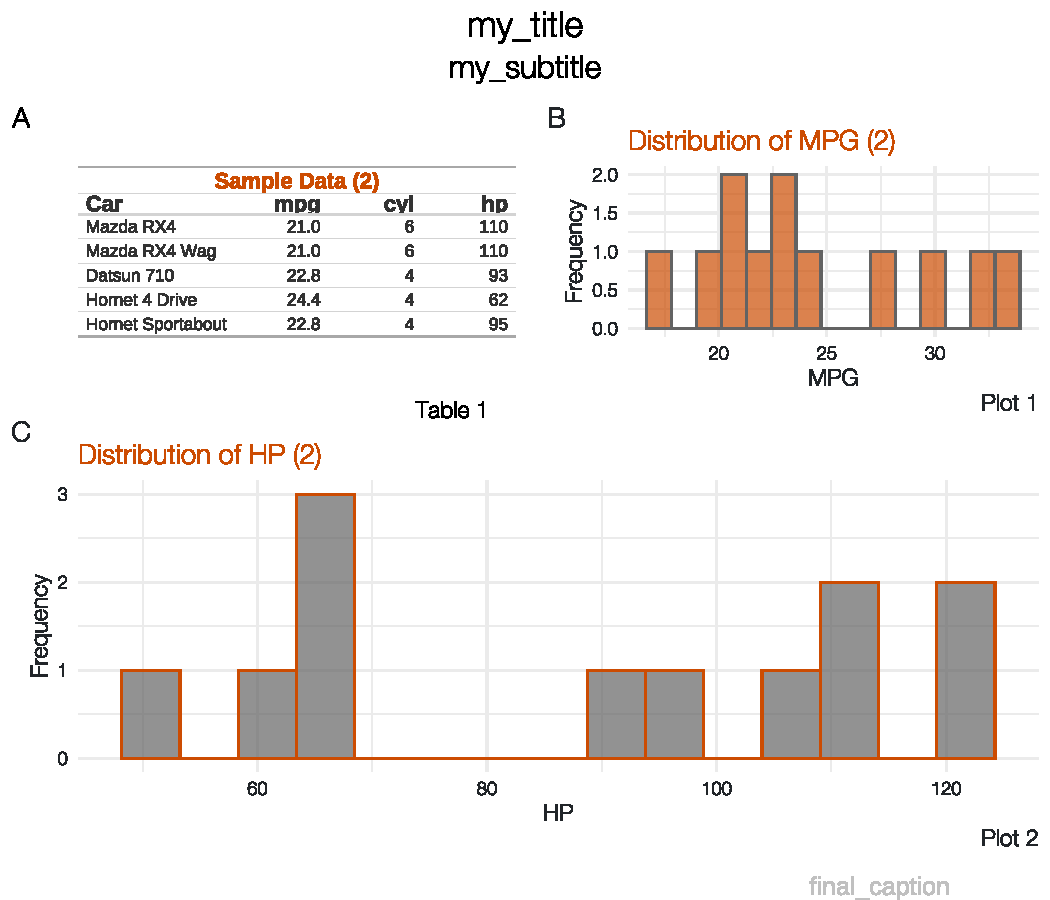
\includegraphics[keepaspectratio]{pdf_11_files/figure-pdf/fig-A-1-1.pdf}}

}

\caption{\label{fig-A-1}}

\end{figure}%

See Fig.~\ref{fig-A-1}.

\pandocbounded{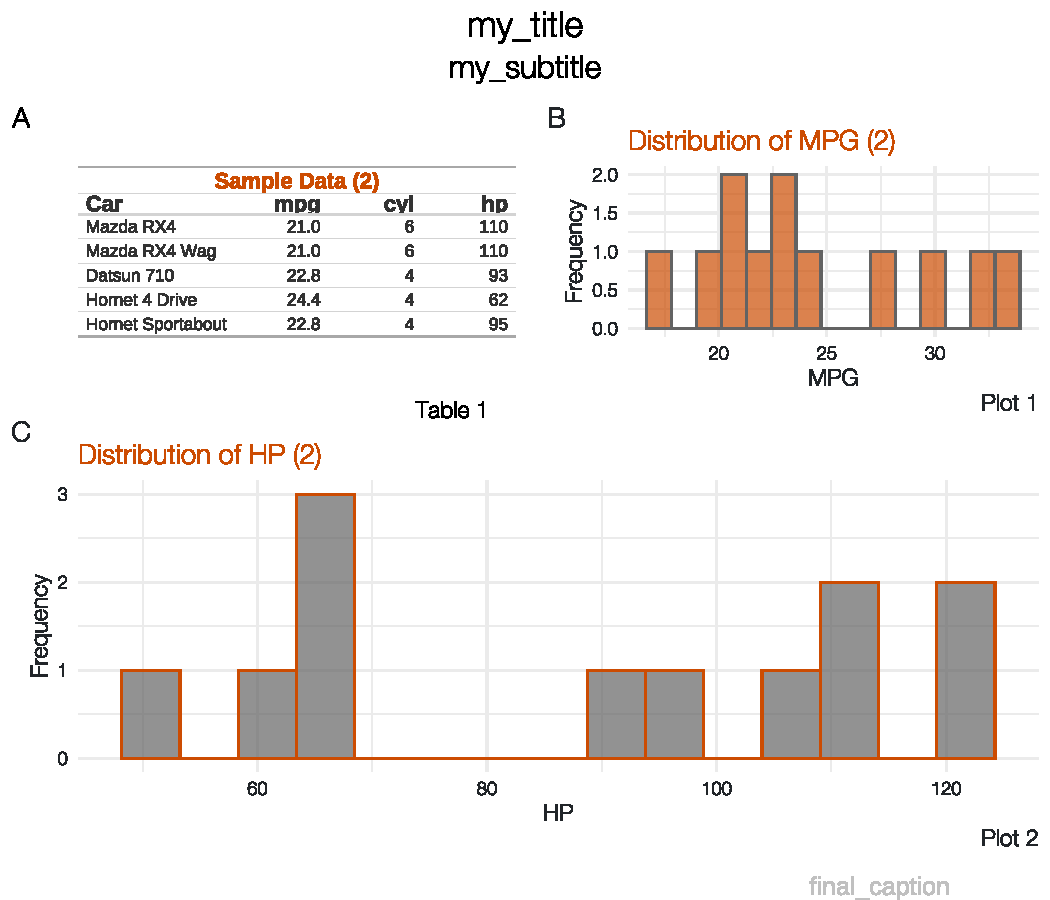
\includegraphics[keepaspectratio]{pdf_11_files/figure-pdf/Plot A.I-1.pdf}}

See (\citeproc{ref-Plot}{\textbf{Plot?}}) A.I.

\subsection{Plot B Visualizations}\label{plot-b-visualizations}

\begin{verbatim}
$plot_B_n
[1] 2

$plot_B_x1
[1] "4"

$plot_B_annotation_1_1
[1] "fig-B-1"

$plot_B_annotation_1_2
[1] "Plot B.I"

$plot_B_annotation_1_3
[1] "Figure I Analysis"

$plot_B_annotation_1_4
[1] "Panel B.I.1"

$plot_B_annotation_1_5
[1] "Panel B.I.2"

$plot_B_annotation_1_6
[1] "Panel B.I.3"

$plot_B_annotation_1_7
[1] "Panel B.I.4"

$plot_B_annotation_1_8
[1] "Figure B.I"

$plot_B_x2
[1] "4"

$plot_B_annotation_2_1
[1] "fig-B-2"

$plot_B_annotation_2_2
[1] "Plot B.II"

$plot_B_annotation_2_3
[1] "Figure II Analysis"

$plot_B_annotation_2_4
[1] "Panel B.II.1"

$plot_B_annotation_2_5
[1] "Panel B.II.2"

$plot_B_annotation_2_6
[1] "Panel B.II.3"

$plot_B_annotation_2_7
[1] "Panel B.II.4"

$plot_B_annotation_2_8
[1] "Figure B.II"

$plot_B_Notes_shared
[1] ""

$plot_B_caption_shared
[1] ""
\end{verbatim}

\begin{figure}

\centering{

\pandocbounded{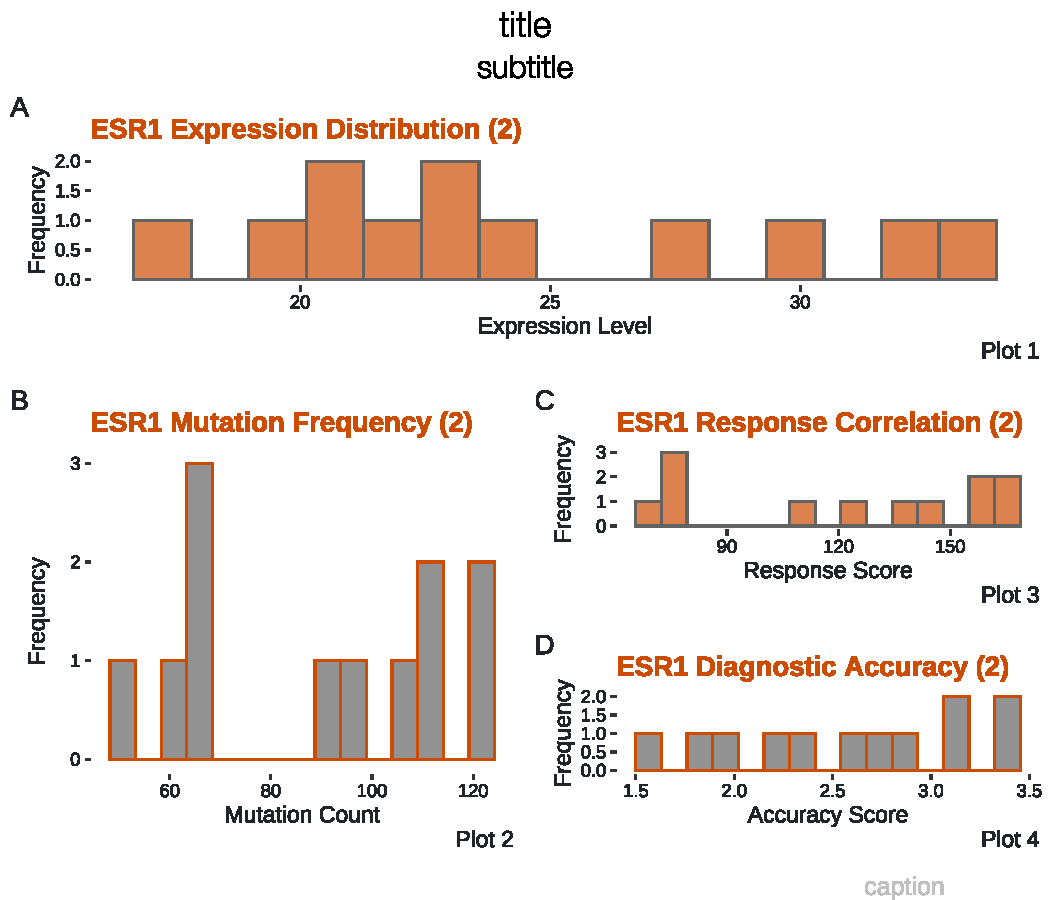
\includegraphics[keepaspectratio]{pdf_11_files/figure-pdf/fig-B-1-1.pdf}}

}

\caption{\label{fig-B-1}}

\end{figure}%

See Fig.~\ref{fig-B-1}.

\pandocbounded{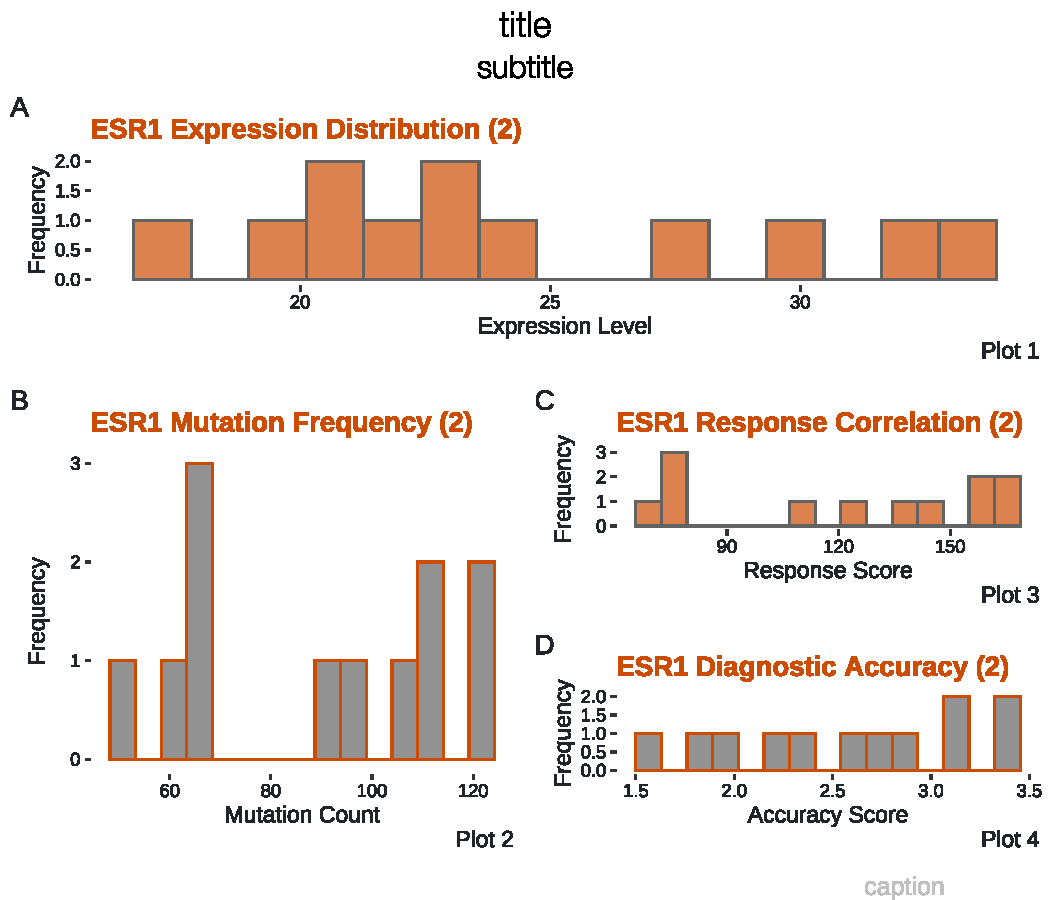
\includegraphics[keepaspectratio]{pdf_11_files/figure-pdf/Plot B.I-1.pdf}}

See (\citeproc{ref-Plot}{\textbf{Plot?}}) B.I.


\backmatter


\end{document}
